%%%%%%%%%%%%%%%%%%%%%%%%%%%%%%%%%%%%%%%%%
% Developer CV
% LaTeX Template
% Version 1.0 (28/1/19)
%
% This template originates from:
% http://www.LaTeXTemplates.com
%
% Authors:
% Jan Vorisek (jan@vorisek.me)
% Based on a template by Jan Küster (info@jankuester.com)
% Modified for LaTeX Templates by Vel (vel@LaTeXTemplates.com)
%
% License:
% The MIT License (see included LICENSE file)
%
%%%%%%%%%%%%%%%%%%%%%%%%%%%%%%%%%%%%%%%%%

%----------------------------------------------------------------------------------------
%	PACKAGES AND OTHER DOCUMENT CONFIGURATIONS
%----------------------------------------------------------------------------------------

\documentclass[9pt]{developercv} % Default font size, values from 8-12pt are recommended

%----------------------------------------------------------------------------------------

\begin{document}

%----------------------------------------------------------------------------------------
%	TITLE AND CONTACT INFORMATION
%----------------------------------------------------------------------------------------

\begin{minipage}[t]{0.45\textwidth} % 45% of the page width for name
	\vspace{-\baselineskip} % Required for vertically aligning minipages

	% If your name is very short, use just one of the lines below
	% If your name is very long, reduce the font size or make the minipage wider and reduce the others proportionately
	{\HUGE\textcolor{black}{\textbf{\MakeUppercase{Sven}}}} % First name

	{\HUGE\textcolor{black}{\textbf{\MakeUppercase{Rademakers}}}} % Last name

	\vspace{6pt}

    {\huge Senior Software Engineer} % Career or current job title
\end{minipage}
\begin{minipage}[t]{0.31\textwidth} % 27.5% of the page width for the first row of icons
	\vspace{-\baselineskip} % Required for vertically aligning minipages

	% The first parameter is the FontAwesome icon name, the second is the box size and the third is the text
	% Other icons can be found by referring to fontawesome.pdf (supplied with the template) and using the word after \fa in the command for the icon you want
	\icon{MapMarker}{12}{Portslade, UK}\\
	\icon{Phone}{12}{+44 (0)7 411 968 492}\\
	\icon{At}{12}{\href{mailto:sven.rademakers@gmail.com}{sven.rademakers@gmail.com}}\\
\end{minipage}
\begin{minipage}[t]{0.275\textwidth} % 27.5% of the page width for the second row of icons
	\vspace{-\baselineskip} % Required for vertically aligning minipages

	% The first parameter is the FontAwesome icon name, the second is the box size and the third is the text
	% Other icons can be found by referring to fontawesome.pdf (supplied with the template) and using the word after \fa in the command for the icon you want
    %	\icon{Globe}{12}{\href{https://svenrademakers.com}{svenrademakers.com}}\\
	\icon{Linkedin}{12}{\href{https://www.linkedin.com/in/sxrademakers}{sxrademakers}}\\
	\icon{Github}{12}{\href{https://github.com/svenrademakers}{svenrademakers}}\\
\end{minipage}
%----------------------------------------------------------------------------------------
%	INTRODUCTION, SKILLS AND TECHNOLOGIES
%----------------------------------------------------------------------------------------


\cvsect{Who Am I?}
\begin{minipage}[t]{0.2\textwidth} % 50% of the page for the skills bar chart
	\vspace{0.5em} % Required for vertically aligning minipages
    \setlength{\fboxsep}{0pt}%
    \setlength{\fboxrule}{1pt}%
    \fbox{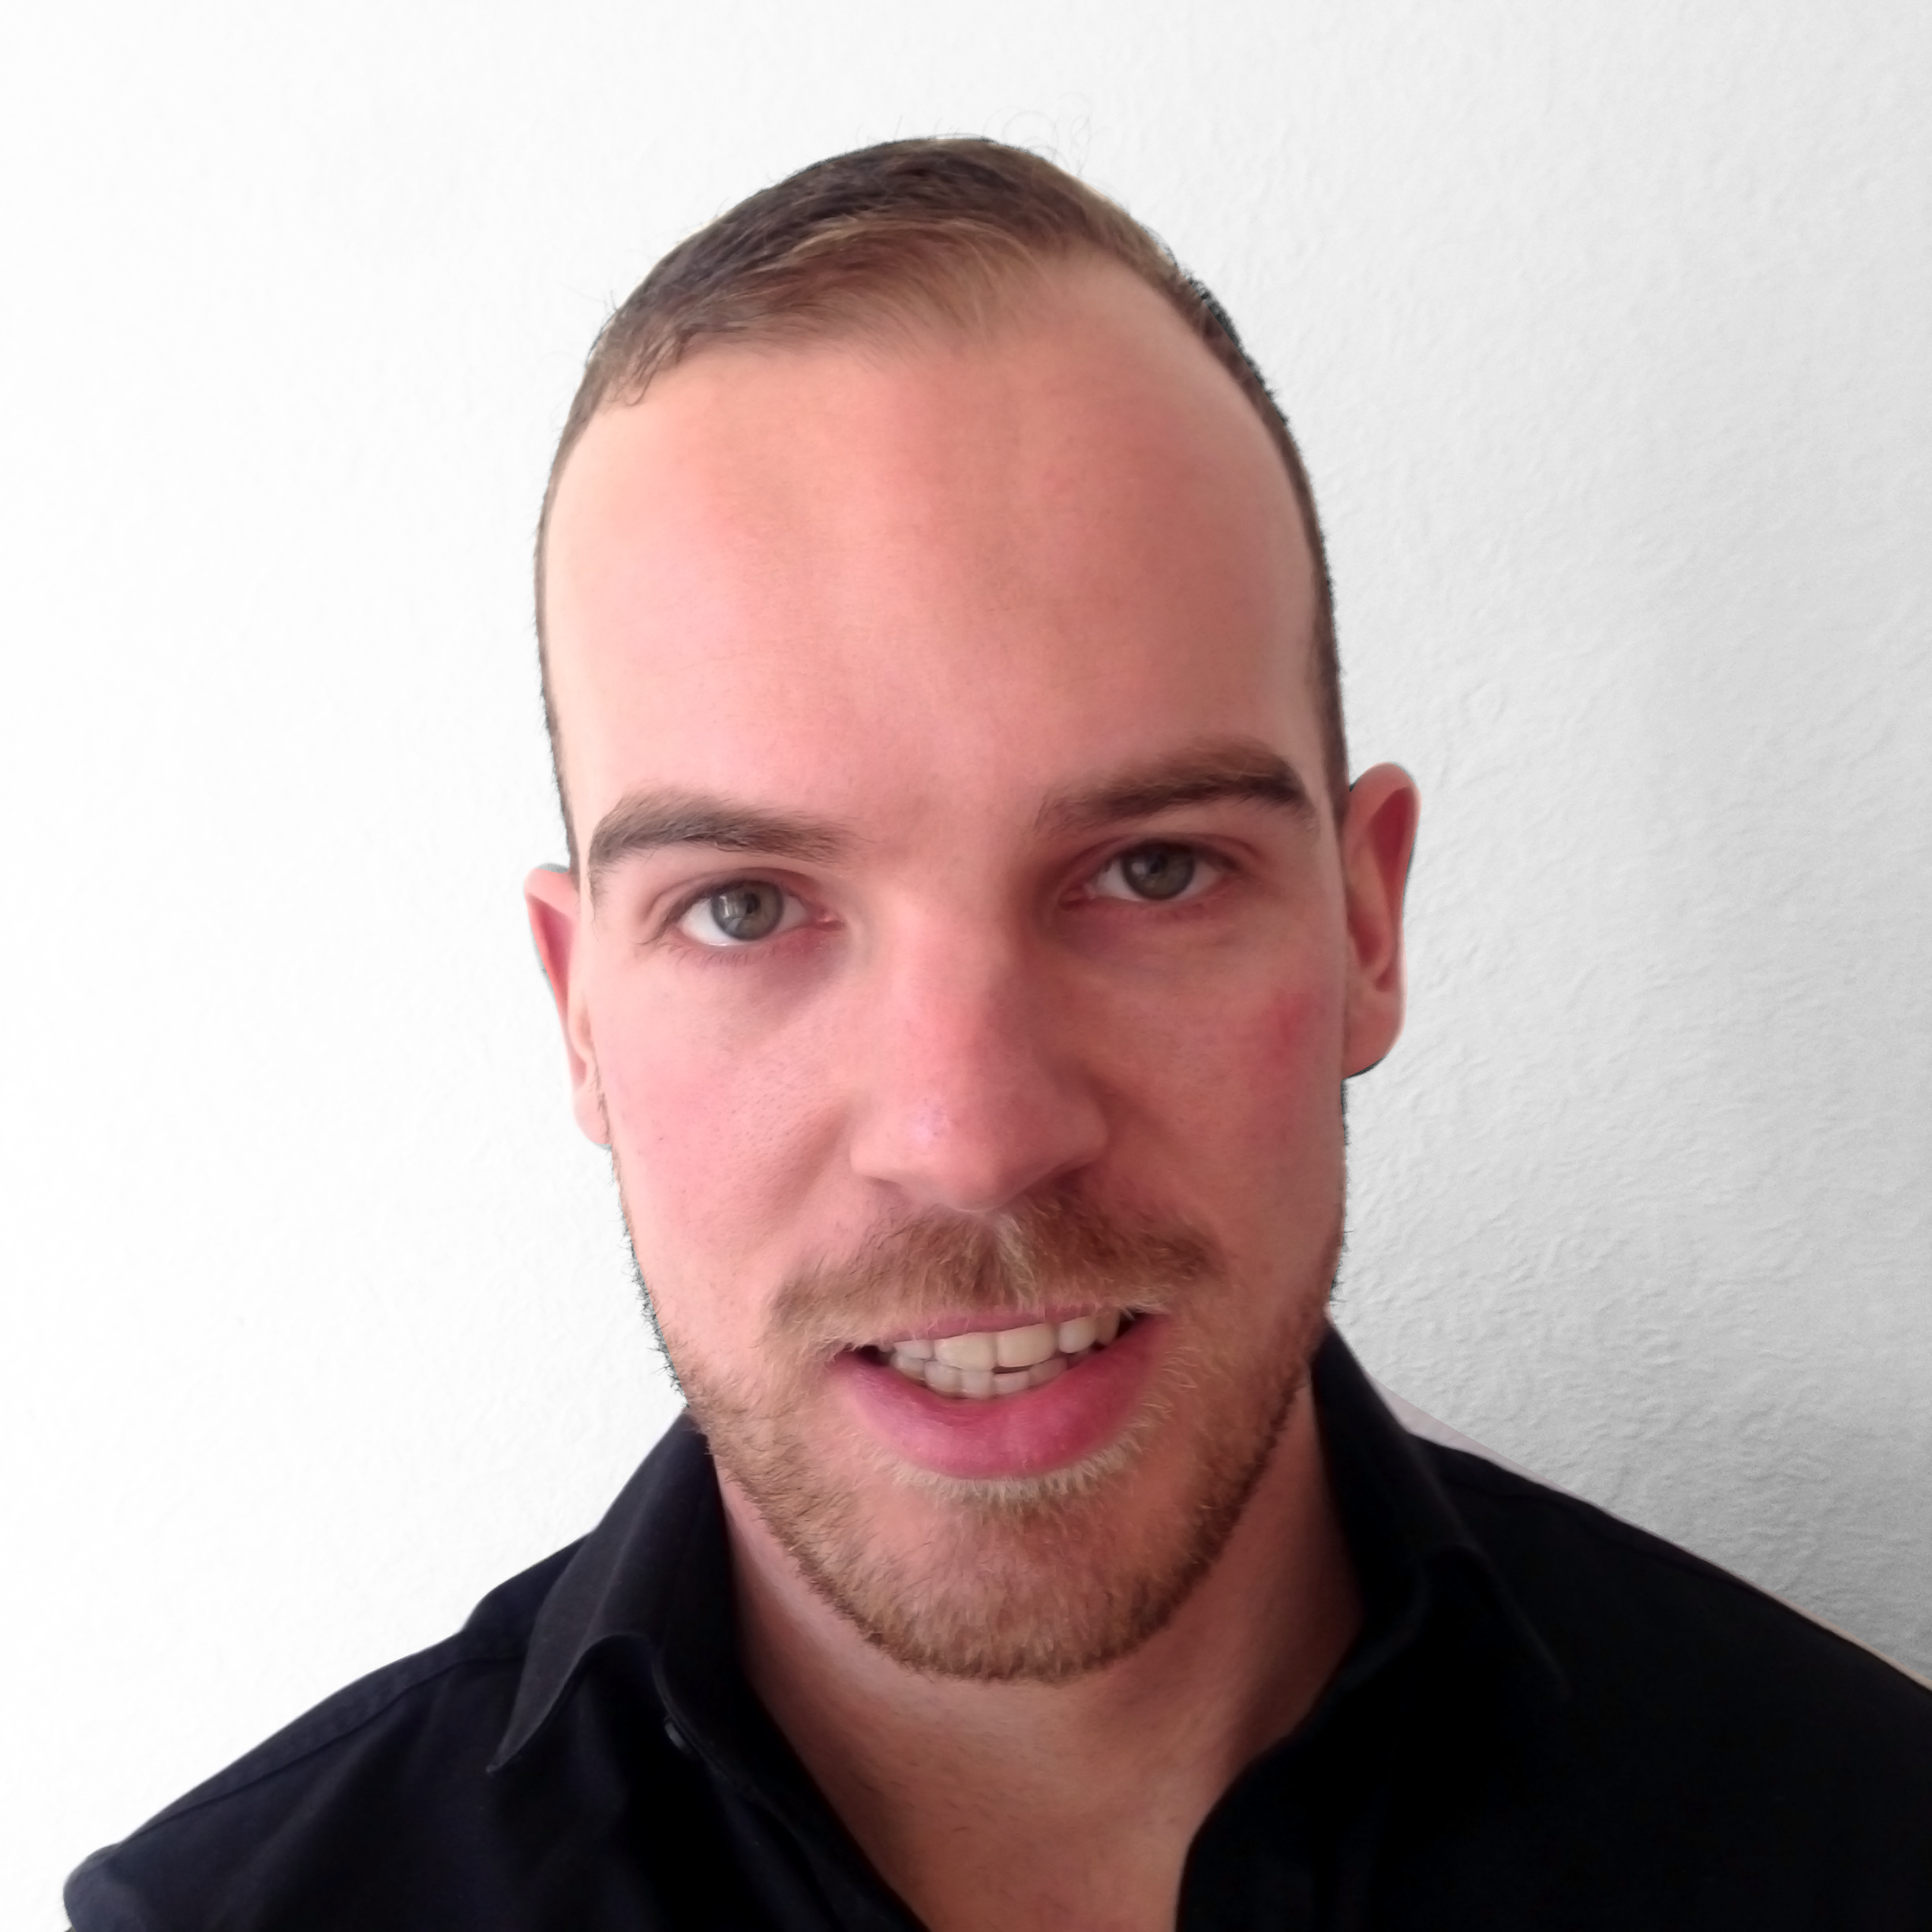
\includegraphics[height=4cm]{Sven.png}}
\end{minipage}
\hspace{3.5em}
\begin{minipage}[t]{0.7\textwidth} % 40% of the page width for the introduction text
	\vspace{0.5em} % Required for vertically aligning minipages


    \colorbox{black}{\textcolor{white}{Experience:}}
    \colorbox{black}{\textcolor{white}{Rust 4 years}}
    \colorbox{black}{\textcolor{white}{C++ 7 years}}
    \newline{}
    \colorbox{black}{\textcolor{white}{Nationality: Netherlands}}
    \colorbox{black}{\textcolor{white}{UK Visa: PBS Dependant}}
    \newline{}
    \colorbox{black}{\textcolor{white}{Age: 33 years}}
    \newline{}
    \newline{}
     Driven to expand my expertise in Low level systems, embedded, Linux, and concurrency. Very curious by nature, always seeking to learn new things and I never back down from a challenge.\newline{}
    A successful project for me is when we took calculated risks, pushed the
    envelope on technology, while staying realistic.
    \newline{}
    \texttt{Trust}\slashsep\texttt{Communication}\slashsep\texttt{Transparency}\slashsep\texttt{Perseverance}
\end{minipage}
%----------------------------------------------------------------------------------------
%	EXPERIENCE
%----------------------------------------------------------------------------------------

\cvsect{Experience}
\begin{entrylist}
	\entry
        {\cvdate{April 2023} {August 2024} }
		{Lead Rust Engineer}
        {London, UK\\Turing Machines}
		{Architected, implemented and deployed firmware based on embedded linux
        for the Turing Pi platform, A compact edge cluster.
        \begin{itemize}
           \setlength\itemsep{-0.5em}
               \item {Laid down the vision and foundation for the product.}
               \item {Setup embedded linux kernel and factory automation images}
               \item {Designed and implemented a system to stream OS images to the inserted compute modules via a web UI.}
                \item {Implemented a bootloader SPL that boots the appropriate DTS tree based on EEPROM content}
          \end{itemize}
        \texttt{u-boot}\slashsep\texttt{buildroot}\slashsep\texttt{cortex-A7}\slashsep\texttt{Linux}\slashsep\texttt{C}\slashsep\texttt{dts}\slashsep\texttt{Rust}\slashsep\texttt{actix}\slashsep\texttt{tokio}
        }
	\entry
        {\cvdate{March 2023}{Nov 2020}}
		{Senior Software Engineer}
        {Copenhagen, Denmark\\Silicon Labs}
		{Part of IoT gateway SDK team. This SDK is a platform that connects Z-Wave, Zigbee, Bluetooth protocol stacks to specific back-ends in an unified way. As a Rust lead my objective was to increase rust expertise in the company and grow the Rust code base.
          \begin{itemize}
           \setlength\itemsep{-0.5em}
                \item {Implemented features in Rust using tokio, no\_std, FFI, proc-macros.}
        		\item {Release Coordinator. End responsible in making sure releases are according quality and delivered on time to our customers.}
                \item {Designed and implemented a build-system that compiles Rust into C++ code bases using FFI.}
        		\item {Designed and implemented procedural macros that simplifies data marshalling between Rust and C code.}
        		\item {Designed and implemented custom async runtime in Rust on top of contiki (resource constrained OS).}
          \end{itemize}
        \texttt{Rust}\slashsep\texttt{tokio}\slashsep\texttt{no\_std}\slashsep\texttt{tauri}\slashsep\texttt{proc-macros}\slashsep\texttt{linux}\slashsep\texttt{arm64}\slashsep\texttt{nix}\slashsep\texttt{docker}\slashsep\texttt{C++}\slashsep\texttt{git}\slashsep\texttt{python}\slashsep\texttt{bash}
        }
	\entry
		{\cvdate{Nov 2020}{Jan 2018}}
		{Snowdrop Programmer}
		{Malmo, Sweden\\Massive Entertainment, a Ubisoft studio}
		{Member of the snowdrop team as programmer. (C++/Visual Studio) Game engine used for Tom Clancy's The Division 2.
          \begin{itemize}
           \setlength\itemsep{-0.5em}
            \item { Developed Asset Mover tool in snowdrop editor (C++). packing of data, dependency-tracking, asset management.}
            \item { Designed and implemented features for GENIE, a cut scene editor of snowdrop. (concurrency, C++) }
            \item { Supported sharpmake. in-house solution for generating build and
                project files. }
         \end{itemize}
        \texttt{C++}\slashsep\texttt{snowdrop}\slashsep\texttt{Visual Studio}\slashsep\texttt{windows}\slashsep\texttt{perforce}\slashsep\texttt{sharpmake}
        }
	\entry
		{\cvdate{Jan 2018}{Feb 2016}}
        {Embedded Software Engineer}
        {Eindhoven, the Netherlands\\Philips}
        {Developed Philips connectivity firmware on cypress microchips, Cortex-M4.(C++/ C, FreeRTOS, NetX)
          \begin{itemize}
           \setlength\itemsep{-0.5em}
            \item {Implemented features related to WIFI domain: UDP, TCP/IP, HTTP, TLS, SSDP.}
            \item {Developed a Philips proprietary protocol based on SPI, UART and HTTP transports.}
            \item {Implemented a streaming protocol on top of BLE GATT profile.}
            \item {Migrated legacy C code to C++.}
            \item {Developing and maintaining test automation (C\#).}
            \item {Developing EmbeddedInfralib. a STL lookalike lib designed for embedded systems.}
            \item {Created build automation and CI tooling (Python).}
          \end{itemize}
        \texttt{C++}\slashsep\texttt{cortex-M}\slashsep\texttt{docker}\slashsep\texttt{git}\slashsep\texttt{cmake}
        }
	\entry
		{\cvdate{Jan 2016}{Feb 2013}}
        {Software Engineer}
        {Eindhoven, the Netherlands\\TomTom Automotive}
        {Developed Linux based navigation software for an in-dash car system using QT framework.
         \begin{itemize}
           \setlength\itemsep{-0.5em}
            \item {implemented GENIVI navigation services communicating over DBUS.}
            \item {Implemented tacho and gyro filters for more reliable positioning of the car. }
            \item {Lead on performance and stabilization. Profiled and improved 1.start-up behaviour, 2.performance, 3.memory usage, using profilers (valgrind) and memory leak detectors.}
            \item {Fixed and stabilized Multithreading and mapviewer issues.}
          \end{itemize}
        \texttt{C++}\slashsep\texttt{android}\slashsep\texttt{cmake}\slashsep\texttt{linux}\slashsep\texttt{git}\slashsep\texttt{Qt}
        }
\end{entrylist}

%----------------------------------------------------------------------------------------
%	EDUCATION
%----------------------------------------------------------------------------------------

\cvsect{Education}

\begin{entrylist}
	\entry
		{2009 -- 2013}
		{Bachelor of computer science}
        {Fontys University of Applied Sciences}
        {Minor in embedded systems}
\end{entrylist}

%----------------------------------------------------------------------------------------
%	ADDITIONAL INFORMATION
%----------------------------------------------------------------------------------------

\begin{minipage}[t]{0.3\textwidth}
	\vspace{-\baselineskip} % Required for vertically aligning minipages
	\cvsect{Languages}

	\textbf{Dutch} - native\\
	\textbf{English} - proficient\\
\end{minipage}\\\\\\
\begin{minipage}[t]{0.3\textwidth}
	\vspace{-\baselineskip} % Required for vertically aligning minipages
	\cvsect{Hobbies}

	Next to software engineering one of my hobbies is playing guitar and doing sports (cycling).
\end{minipage}

%----------------------------------------------------------------------------------------

\end{document}
